\section{Binary State Vectors}

I consider here the case where a state consists of a finite $D$-dimensional 
binary vector, $\ell_j$, the emission parameter vector $\theta_j$ is all of $\ell_j$, and the emission distribution is based on a noisy linear transformation of the state vector according to a $D \times K$ weight matrix $W$, so that each $K$-dimensional
observation is $\Norm{W^{\sf T} \theta_j}{\Sigma}$.  For the experiments discussed
in this chapter, I will assume that $\Sigma$ does not depend on $j$, but this assumption
is easily relaxed if appropriate.  For finite-length binary vector
states, the set of possible states is finite, and so on its face it may
seem that a nonparametric model is unnecessary.  However, if $D$ is
reasonably large, it is likely that most of the $2^D$ possible states
are vanishingly unlikely (and, in fact, the number of observations may
well be less than $2^D$), and so we would like a model that encourages
the selection of a sparse set of states.  Moreover, there could be more
than one state with the same emission parameters, but with different transition
dynamics. 

We require a similarity function, $\phi(\theta_j, \theta_{j'})$, which 
varies between 0 to 1, and is equal to 1 if and only if $\theta_j =
\theta_{j'}$.  A natural choice in this setting is the Laplacian kernel:
\begin{align}
  \label{eq:39}
  \phi_{jj'} &= \phi(\theta_j, \theta_{j'}) = \exp(-\lambda \Delta_{jj'})
\end{align}
where $\Delta_{jj'd} = \abs{\theta_{jd} - \theta_{j'd}}$, $\Delta_{jj'} =
\sum_{d=1}^D \Delta_{jj'}$ is the Hamming
distance between $\theta_j$ and $\theta_{j'}$,
and $\lambda \geq 0$ (if $\lambda = 0$, the $\phi_{jj'}$
are all 1, and so do not have any influence, reducing the
model to an ordinary HDP-HMM).

Before describing individual experiments, I describe the additional
inference steps needed for these variables.

\subsection{Additional Inference Steps}
\label{sec:sampling-eta}

\paragraph{Sampling $\theta$} We put independent Beta-Bernoulli priors
on each coordinate of $\theta$.  Each coordinate $\theta_{jd}$ can be sampled
conditioned on all the others and the coordinate-wise prior means,
$\{\mu_d\}$, which we sample in turn conditioned on the $\theta$s.  Since individual coordinates are binary, each one has a Bernoulli posterior, whose parameter we now derive by computing the posterior log-odds, that is we will derive
\begin{equation}
  \label{eq:1}
  \log \frac{p(\theta_{jd} = 1 \given \theta\setminus\theta_{jd}, z, Q, Y)}{p(\theta_{jd} = 0 \given \theta\setminus\theta_{jd}, z, Q, Y)}
\end{equation}
Since $\theta_{jd}$ affects both the similarity matrix and the emission distribution, the posterior log-odds has three components: 
the prior log odds, the likelihood due to the successful and failed transitions (specifically the outgoing transition counts from state $j$, $n_{jj'}$ and $q_{jj'}$, as well as the incoming transition counts to state $j$, $n_{j'j}$ and $q_{j'j}$, across all $j'$), 
and the likelihood due to the data, $y$, for those $t$ such that $z_{t} = j$.

The prior log odds is simply $\log(\mu_d / (1 - \mu_d))$.  Next, we compute the likelihood component due to the transition attempts, that is
\begin{equation*}
  \log \frac{p(z, Q \given \theta_{jd} = 1, \theta\setminus\theta_{jd}, \lambda)}{p(z, Q \given \theta_{jd} = 0, \theta\setminus\theta_{jd}, \lambda)}
\end{equation*}

Let
\begin{align}
  \label{eq:68}
  \phi_{jj'-d} &= \exp(-\lambda(\Delta_{jj'} - \Delta_{jj'd}))
\end{align}
so that $\phi_{jj'} = \phi_{jj'-d} e^{-\lambda\Delta_{jj'd}}$.

Since the matrix $\phi$ is assumed to be symmetric, we have
\begin{align}
  \label{eq:70}
  \frac{p(z, Q \given \theta_{jd}  = 1, \theta\setminus\theta_{jd}
    )}{p(z, Q \given \theta_{jd}  = 0, \theta\setminus\theta_{jd} )}
  &\propto \prod_{j' \neq j}
  \frac{e^{-\lambda(n_{jj'} + n_{j'j})\abs{1 - \theta_{j'd}}}(1 -
    \phi_{jj'-d} e^{-\lambda\abs{1 - \theta_{j'd}}})^{q_{jj'} +
      q_{j'j}}}{e^{-\lambda(n_{jj'} + n_{j'j})\abs{\theta_{j'd}}}
    (1-\phi_{jj'-d}e^{-\lambda\abs{\theta_{j'd}}})^{q_{jj'} +
      q_{j'j}}} \\
  &= \label{eq:71} e^{-\lambda(c_{jd0} - c_{jd1})}
  \prod_{j' \neq j} \left(\frac{1 - \phi_{jj'-d}e^{-\lambda}}{1-\phi_{jj'-d}}\right)^{(-1)^{\theta_{j'd}}(q_{jj'} + q_{j'j})}
\end{align}
where $c_{jd0}$ and $c_{jd1}$ are the number of successful jumps to or
from state $j$, to or from states with a 0 or 1, respectively, in
position $d$.  That is,
\begin{equation}
  \label{eq:72}
  c_{jd0} = \sum_{\{j' \given \theta_{j'd} = 0\}} n_{jj'} + n_{j'j}\qquad c_{jd1} = \sum_{\{j' \given \theta_{j'd} = 1\}} n_{jj'} + n_{j'j}
\end{equation}

We assume the observed data $Y$ consists of a $T \times K$
matrix, where the $t$th row $y_t = (y_{t1}, \dots,
y_{tK})$ is a $K$-dimensional feature vector associated
with time $t$, and let $W$ be a $D \times K$ weight matrix
with $k$th column $w_k$ that maps $D$ dimensional binary state vectors 
to means in the $K$-dimensional observation space.  Then
the part of the likelihood function from time $t$ is
\begin{equation}
  \label{eq:74}
  p(y_t \given z_t, \theta_{z_t}) = \Norm{y_t \given W^{\sf T}\theta_{z_t}}{\Sigma}
\end{equation}
In the experiments discussed here, $\Sigma$ is asssumed diagonal with entries $\sigma^2_k$, $k = 1, \dots, K$, and does not depend on $j$.  Under this assumption, we have
\begin{equation}
  \label{eq:73}
  p(y_t \given W^{\mathsf{T}} \theta_{z_t}) = \prod_{k=1}^K \Norm{y_t \given w_k^{\sf T}\theta_{z_t}}{\sigma^2_k}.
\end{equation}
The coordinate $\theta_{jd}$ affects the likelihood only through the mean, $W^{\sf T} \theta_j$.  Expanding this mean to isolate the effect of $\theta_{jd}$, we have
\begin{equation*}
  w_k^{\sf T}\theta_j = \sum_{d} w_{dk} \theta_{jd}
\end{equation*}
and so we see that setting $\theta_{jd} = 1$ vs 0 shifts the $k$th coordinate 
of the mean, $W_{\sf T} \theta_{j}$, by $w_{dk}$.  Denote by $\theta^*$ the matrix 
whose $t$th row consists of the binary state vector $\theta_{z_t}$, and 
let $X^* = W^{\sf T} \theta^*$.  As shorthand, write $x_{tk}^{(-d)}$ to be the $(t,k)$ entry in $X^*$ assuming that $\theta_{jd} = 0$. Then the corresponding value if $\theta_{jd} = 1$ is $x_{tk}^{(-d)} + w_{dk}$. Since the $y_t$ are conditionally independent given the state sequence, $z$, we can write the log likelihood ratio for $\theta_{jd} = 1$ versus $\theta_{jd} = 0$ as
\begin{equation}
  \label{eq:91}
  \sum_{t: z_t = j} \sum_{k=1}^K\log\left(\frac{\Norm{y_{tk} \given
    x_{tk}^{(-d)} + w_{dk}}{\sigma^2_k})}{\Norm{y_{tk} \given
    x_{tk}^{(-d)}}{\sigma^2_k}}\right) = \sum_{t: z_t = j} \sum_{k=1}^K -\frac{w_{dk}}{\sigma^2_k}(y_{tk} - x_{tk}^{(-d)} + \frac{1}{2}w_{dk})
\end{equation}

All together, we have
\begin{align}
  \label{eq:77}
  &\log\left(\frac{p(\theta_{jd} = 1 \given Y, z, Q, \theta \setminus
    \theta_{jd})}{p(\theta_{jd} = 0 \given Y, z, Q, \theta
    \setminus \theta_{jd})}\right) \\ &\qquad = \log\left(\frac{p(\theta_{jd} =
  1) p(z, Q \given \theta_{jd} = 1, \theta \setminus
  \theta_{jd}) p(Y \given z, \theta_{jd} = 1, \theta \setminus \theta_{jd})}{p(\theta_{jd} = 0) p(z, Q \given \theta_{jd} = 0,
  \theta \setminus \theta_{jd}) p(Y \given z, \theta_{jd} = 0,
  \theta \setminus \theta_{jd})}\right) \\ & \qquad = \log\left(\frac{\mu_d}{1 - \mu_d}\right)
  \\ & \qquad \qquad + (c_{jd1} - c_{jd0}) \lambda +
    \sum_{j' \neq j}
  (-1)^{\theta_{j'd}}(q_{jj'} + q_{j'j})\log\left(\frac{1 -
      \phi_{jj'}^{(-d)}e^{-\lambda}}{1-\phi_{jj'}^{(-d)}}\right) \\ &
  \qquad \qquad + \sum_{t: z_t = j} \sum_{k=1}^K -\frac{w_{dk}}{\sigma^2_k}(y_{tk} - x_{tk}^{(-d)} + \frac{1}{2}w_{dk})
\end{align}

\paragraph{Sampling $\mu$}
\label{sec:sampling-bmu}

Sampling the $\mu_d$ is straightforward with a Beta prior.  Suppose
\begin{equation}
  \label{eq:92}
  \mu_d \stackrel{ind}{\sim} \Beta{a_\mu}{b_\mu}
\end{equation}
Then, conditioned on $\theta$ the $\mu_d$ are independent with
\begin{equation}
  \label{eq:93}
  \mu_d \given \theta \sim \Beta{a_\mu + \sum_{j} \theta_{jd}}{b_\mu +
  \sum_{j} (1 - \theta_{jd})}
\end{equation}

\paragraph{Sampling $W$ and $\Sigma$}
Conditioned on the state matrix $\theta$ and the data matrix $Y$, 
the weight matrix $W$ can be sampled as well using standard methods
for Bayesian linear regression.  We place a zero mean Normal prior on each
element of $W$ (including a row of intercept terms), resulting in a
multivariate Normal posterior for each column.  For the experiments
reported below, we constrain $\Sigma$ to be a diagonal matrix, and
place an Inverse Gamma prior on the variances, resulting in conjugate updates.

Define the prior:
\begin{equation}
  \label{eq:78}
  p(W) = \prod_{k=1}^K\prod_{d=1}^D \mathcal{N}(w_{dk} \given 0,\sigma^2_0).
\end{equation}
The likelihood is
\begin{equation}
  \label{eq:79}
  p(Y \given W, \theta) = \prod_{t=1}^T \prod_{k=1}^K p(y_{tk}; x_{tk}) = \prod_{t=1}^T \prod_{k=1}^K \mathcal{N}(y_{tk} \given x_{tk},\sigma^2_k)
\end{equation}
Then it is a standard result from Bayesian linear modeling that
\begin{equation}
  \label{eq:80}
  p(W \given \theta, Y) = \prod_{k=1}^K
  \Norm{\left(\sigma_0^{-2} \mathbf{I} + \Sigma^{-1} \theta^{*\mathsf{T}} \theta^*
    \right)^{-1}\Sigma^{-1} \theta^{*\mathsf{T}} Y}{\left(\sigma_0^{-2} \mathbf{I} + \Sigma^{-1} \theta^{*\mathsf{T}} \theta^{*}\right)^{-1}}
\end{equation}

\paragraph{Sampling $\lambda$}
\label{sec:sampling-lambda}
The Laplacian kernel $\phi$ is defined as $\phi(\theta_j, \theta_{j'}) =
e^{-\lambda d(\theta_j,\theta_{j'})}$, where in our case $d$ is
  Hamming distance.  The parameter $\lambda$ governs the connection between $\theta$ and
$\phi$.  Writing \eqref{eq:65} in terms of $\lambda$ and the distance matrix
$\Delta$ gives the likelihood
\begin{equation}
  \label{eq:88}
  p(z, Q \given \lambda, \theta) \propto \prod_{j}\prod_{j'}
  e^{-\lambda \Delta_{jj'} n_{jj'}}(1-e^{-\lambda\Delta_{jj'}})^{q_{jj'}} 
\end{equation}
We put an $\Exp{b_{\lambda}}$ prior on $\lambda$, which yields a
posterior density
\begin{equation}
  \label{eq:88}
  p(\lambda \given z, Q, \theta) \propto
  e^{-(b_{\lambda} + \sum_{j}\sum_{j'} \Delta_{jj'} n_{jj'})\lambda} \prod_{j}\prod_{j'}
  (1-e^{-\lambda\Delta_{jj'}})^{q_{jj'}}
\end{equation}
This density is log-concave, with
\begin{equation}
  \label{eq:90}
  -\frac{d^2\log(p(\lambda \given z, Q,
    \theta))}{d\lambda^2} = \sum_{\{(j,j') \given
    \Delta_{jj'} > 0\}}
  \frac{\Delta_{jj'}^2 q_{jj'}
    e^{\lambda\Delta_{jj'}}}{(e^{\lambda\Delta_{jj'}} - 1)^2} > 0
\end{equation}
and so we can use Adaptive Rejection Sampling \citep{gilks1992adaptive}
to sample from it.  To do this we need to compute the log density and its first derivative, which are given by
\begin{align}
  \label{eq:94}
  h(\lambda) &= 
  -(b_{\lambda} + \sum_{\{(j,j') \given \Delta_{jj'} > 0\}} \Delta_{jj'} n_{jj'})\lambda +
  \sum_{\{(j,j') \given \Delta_{jj'} > 0\}} q_{jj'} \log(1 - e^{-\lambda\Delta_{jj'}}) \\
  h'(\lambda) &= -(b_{\lambda} + \sum_{\{(j,j') \given \Delta_{jj'} > 0\}} \Delta_{jj'}
  n_{jj'}) + \sum_{\{(j,j') \given \Delta_{jj'} > 0\}}
  \frac{q_{jj'}\Delta_{jj'}}{e^{\lambda\Delta_{jj'}} - 1}
\end{align}

\subsection{Summary}
\label{sec:summary}

I have made the following assumptions about the representation of the
hidden states and observed data in this subsection:
(1) States are distinguished via a $D$-dimensional binary parameter vector, $\theta_j$ 
(2) the similarity $\phi$ between states $j$ and $j'$
is the Laplacian kernel with respect to Hamming distance 
between the respective $\theta$ vectors, and has a decay parameter 
$\lambda$, and (3) $Y$ consists of $K$ real-valued
features associated with each time step $t$.  In addition, the following priors are applied:
\begin{align}
\mu_d &\stackrel{i.i.d}{\sim} \Beta{a_{\mu}}{b_{\mu}} \\
\lambda &\sim \Exp{b_{\lambda}} \\
\theta_{jd} \given \mu &\stackrel{ind}{\sim} \Bern{\mu_d} \\
w_{dk} &\stackrel{i.i.d.}{\sim} \Norm{0}{\sigma^2_0} \\
y_{tk} \given W, z, \theta &\stackrel{ind}{\sim} \Norm{w_{k}^{T}\theta_{z_t}}{\Sigma}
\end{align}

I introduce Gibbs blocks corresponding to (1) each $\theta_{jd}$
individually, (2) the vector $\mu$, (3) the decay parameter
$\lambda$, and (4) the weight matrix $W$.
We have conditional posterior distributions
\begin{align}
  \label{eq:101}
  \theta_{jd} \given \theta \setminus \theta_{jd}, z, Q, \mu,
  \lambda, W, Y^* &\sim
  \Bern{\frac{e^{\zeta_{jd}}}{1 + e^{\zeta_{jd}}}} \\
  \mu_d \given \theta, \dots &\stackrel{ind}{\sim} \Beta{a_\mu + \sum_{j} \theta_{jd}}{b_\mu +
  \sum_{j} (1 - \theta_{jd})} \\
p(\lambda \given z, Q, \theta, \dots) &\propto e^{-(b_{\lambda} + \sum_{j}\sum_{j'} \Delta_{jj'} n_{jj'})\lambda} \prod_{j}\prod_{j'}
  (1-e^{-\lambda\Delta_{jj'}})^{q_{jj'}} \\
  W \given \theta, Y, z, \dots &\stackrel{ind}{\sim} \Norm{\left(\sigma_0^{-2} \mathbf{I} + \Sigma^{-1} \theta^{*\mathsf{T}} \theta^*
    \right)^{-1}\Sigma^{-1} \theta^{*\mathsf{T}} Y}{\left(\sigma_0^{-2} \mathbf{I} + \Sigma^{-1} \theta^{*\mathsf{T}} \theta^{*}\right)^{-1}}
\end{align}
where $\Delta_{jj'} = \norm{\theta_j - \theta_j'}_{L_1}$ and
\begin{align}
\zeta_{jd} &= \log\left(\frac{\mu_d}{1 - \mu_d}\right)
  + (c_{jd1} - c_{jd0}) \lambda +
    \sum_{j' \neq j}
  (-1)^{\theta_{j'd}}(q_{jj'} + q_{j'j})\log\left(\frac{1 -
      \phi_{jj'}^{(-d)}e^{-\lambda}}{1-\phi_{jj'}^{(-d)}}\right)
  \notag \\ & \qquad - \sum_{\{t \given z_t = j\}} \sum_{k=1}^K
  \frac{w_{dk}}{\sigma^2_k}(y^*_{tk} - x_{tk}^{(-d)} + \frac{1}{2}w_{dk})
\end{align}
All distributions can be sampled from directly except for $\lambda$, which
requires Adaptive Rejection Sampling, with the equations
\begin{align}
  h(\lambda) &= 
  -(b_{\lambda} + \sum_{\{(j,j') \given \Delta_{jj'} > 0\}} \Delta_{jj'} n_{jj'})\lambda +
  \sum_{\{(j,j') \given \Delta_{jj'} > 0\}} q_{jj'} \log(1 - e^{-\lambda\Delta_{jj'}}) \\
  h'(\lambda) &= -(b_{\lambda} + \sum_{\{(j,j') \given \Delta_{jj'} > 0\}} \Delta_{jj'}
  n_{jj'}) + \sum_{\{(j,j') \given \Delta_{jj'} > 0\}}
  \frac{q_{jj'}\Delta_{jj'}}{e^{\lambda\Delta_{jj'}} - 1}
\end{align}


\section{``Cocktail Party'' Data}

To evaluate the model, we created synthetic data based on a speaker 
diarization/blind source separation task known as the ``cocktail party'' problem.  
In such a task, the observable data consists of one or more audio signals, discretized into $T$ segments, where the signal at time $t$ is assumed to arise from multiple speakers, some subset of whom are speaking.  The inference problem is to recover which speakers are speaking when.  We further assume that speakers are grouped into conversations, and take turns speaking within conversation.  In such a task, there are naively $2^S$ possible
states, where each state indicates which of $S$ speakers is speaking
at a particular time step.  However, due to the conversational grouping, if
at most one speaker in a conversation can be speaking at any given
time (a natural assumption of within-group turn-taking), 
the state space is constrained, with only $\prod_c (s_c + 1)$
states possible (with perhaps a small probability of other combinations occurring due to occasional overlap), where $s_c$ is the
number of speakers in conversation $c$.

For the synthetic cocktail party data, the turn sequence within each conversation is
generated using a Hidden Semi-Markov Model (HSMM) with Poisson distributed state-durations, in which the state sequence had $s_c$ states, with pauses with
shorter Poisson duration inserted between each ``sentence''.  The
states within conversations are then mapped to a binary vector with
$s_c$ entries, where silence is represented by all zeroes, 
and speaker $s$ speaking corresponds to a 1 in position $s$.  
The binary vectors are concatenated across
conversations to yield latent states consisting of length $S$ binary
vectors.  To simulate speakers being recorded by $K$ microphones,
weights mapping speakers to microphones were generated independently from
a $U(0,1)$ distribution, resulting in a $D \times K$ weight matrix,
$W$.  A constant ``background sound level'' parameter for each microphone was added as
well, also $U(0,1)$, and independent $\Norm{0}{\sigma^2_k}$ noise was added
to each time step at microphone $k$.

Transition and emission parameters were generated from conjugate priors
to the Poisson HSMM.  The data set
consisted of four conversations of four speakers each, and 12
microphones, so that $D = 16$, and $K = 12$.  There are therefore
$2^{16} = 65536$ possible binary vector-valued states, but only
$(4+1)^4 = 625$, less than 1\%, can actually occur.  The noise variance $\sigma^2_k$ 
was set to a constant of $1/10$ for all $k = 1, \dots, K$.

We attempted to infer the states
from the data using three models: (1) a binary-state Factorial HMM, in which the
individual binary speaker sequences are modeled as independent a
priori, (2) an ordinary HDP-HMM without local transitions, where the
latent states are binary vectors, and (3) our
HDP-HMM-LT model.  The same linear-Gaussian emission model was employed for all three models; the only difference was the prior on the sequence of binary state vectors.

To simplify interpretation of the results, the weight matrix
was fixed to the true value (this makes the latent dimensions
identifiable and makes comparisons between inferred and ground truth
state matrices meaningful).  Each model was evaluated at each Gibbs
iteration using the Hamming distance between inferred 
and ground truth state matrices, as well as the F1 score, which is the harmonic mean between the precision (the proportion of the 1s in the inferred state matrix that were actually 1 in the ground truth) and recall (the proportion of the 1s in the ground truth state matrix that were correctly classified as 1 by the model).

The results for the three models are in Figure
\ref{fig:cocktail-results}.  % In Fig \ref{fig:binary-matrix}, we also plot the ground truth state
% matrix against the expected state matrix for the two HDP models, averaged over the 10 runs and all iterations
% 500 through 1000.  
The LT model outperforms the other two on
all measures on all datasets. 

We also plot the inferred decay rate $\lambda$ for the
HDP-HMM-LT model.  The LT model settles on a non-negligible $\lambda$
value for this data, suggesting that the local transition structure
explains the data well.  It also uses more components than the non-LT
model, perhaps owing to the fact that the weaker transition prior of
the non-LT model is more likely to explain nearby similar observations
as a single persisting state, whereas the LT model places a higher
probability on transitioning to a new state with a similar latent vector.


\begin{figure}[tb]
  \centering
  \begin{minipage}{0.40\textwidth}
  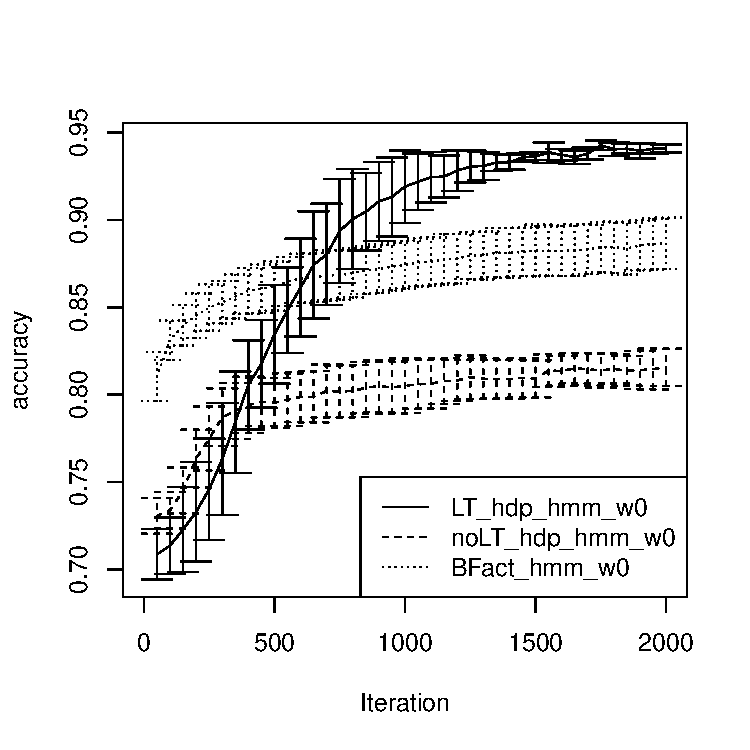
\includegraphics[width = \textwidth]{fig/cocktail_s16_m12/w0/h10.0_nocs_cp1/accuracy.pdf}
\end{minipage}
\hspace{0.1in}
\begin{minipage}{0.40\textwidth}
  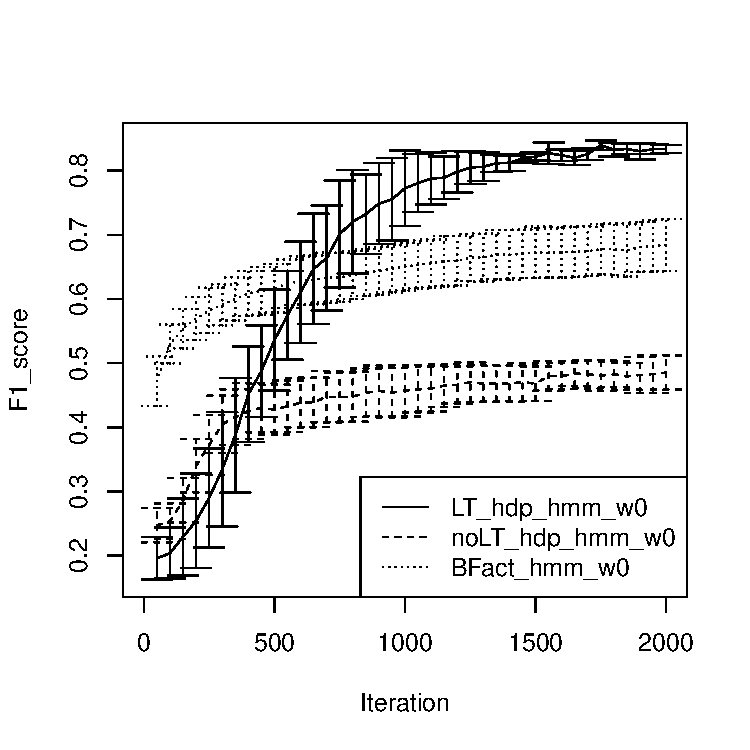
\includegraphics[width = \textwidth]{fig/cocktail_s16_m12/w0/h10.0_nocs_cp1/F1_score.pdf}
\end{minipage}
\vspace{-0.3in}

\begin{minipage}{0.40\textwidth}
  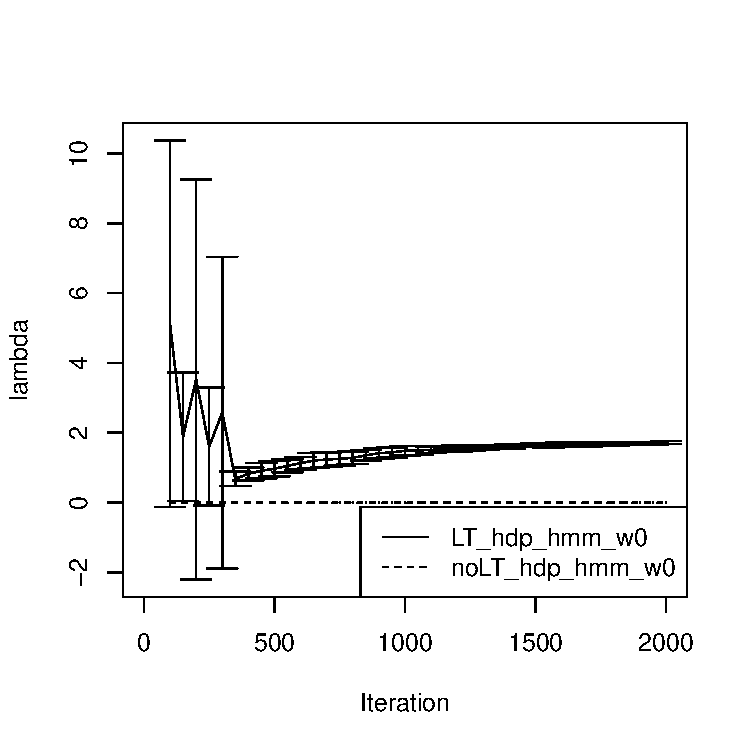
\includegraphics[width = \textwidth]{fig/cocktail_s16_m12/w0/h10.0_nocs_cp1/lambda.pdf}
\end{minipage}
\begin{minipage}{0.40\textwidth}
  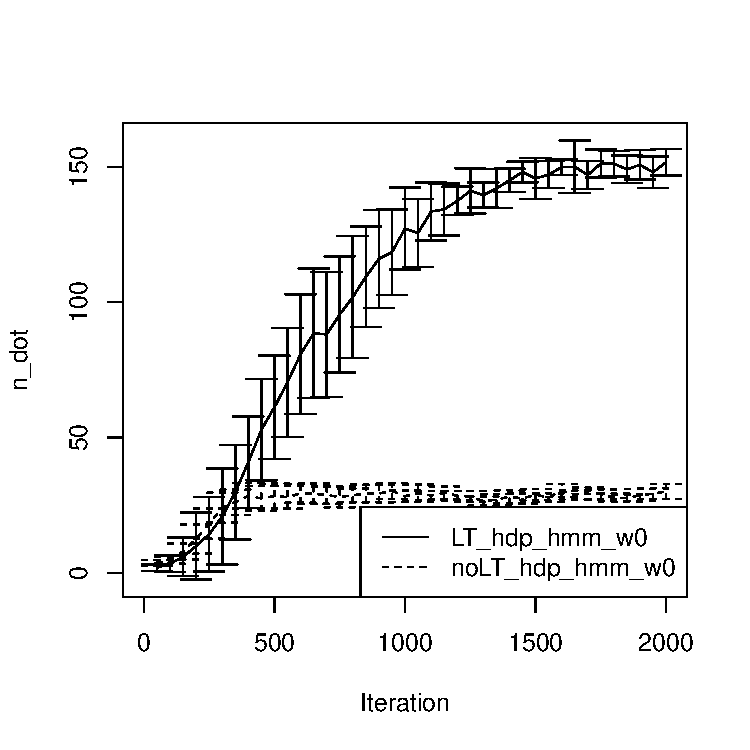
\includegraphics[width = \textwidth]{fig/cocktail_s16_m12/w0/h10.0_nocs_cp1/n_dot.pdf}
\end{minipage}
\caption{(a-b) Accuracy and F1 scores for the HDP-HMM-LT, standard HDP-HMM, and
    Binary Factorial HMM on
    the Cocktail Party Data.  Metrics are averaged
  over 10 Gibbs runs on each model, with error bars representing a 99\% confidence
  interval for the mean per iteration.  The first 100 iterations are
  not shown. (c) Learned similarity parameter, $\lambda$, for the LT
  model, (d) Number of distinct states used by HDP-HMM and
  HDP-HMM-LT.  The first 100 iterations are excluded.}
  \label{fig:cocktail-results}
\end{figure}

\section{Synthetic Data Without Local Transitions}
\label{sec:synth-data-without}

As a ``sanity check'' on the model, data was also generated 
directly from an ordinary HDP-HMM, with no local
transition property, in order to investigate the performance of our
model in a case where the data did not have the key property that its
prior equipped it to discover.  The results are in
Fig. \ref{fig:synthetic-results}.
During iterations when the $\lambda$ parameter is large, the LT model has worse
performance than the non-LT model on this data, as its bias toward
local transitions is not helpful; however, the
$\lambda$ parameter settles near zero as sampling continues, and the 
model learns that a preference for local transitions does not help to explain
the data.  Note that when $\lambda = 0$, the HDP-HMM-LT reduces to an ordinary HDP-HMM.
Unlike on the cocktail party data, the LT model does not use more
states when the data does not have the LT property.

\begin{figure}[tb]
  \centering
  \begin{minipage}{0.40\textwidth}
  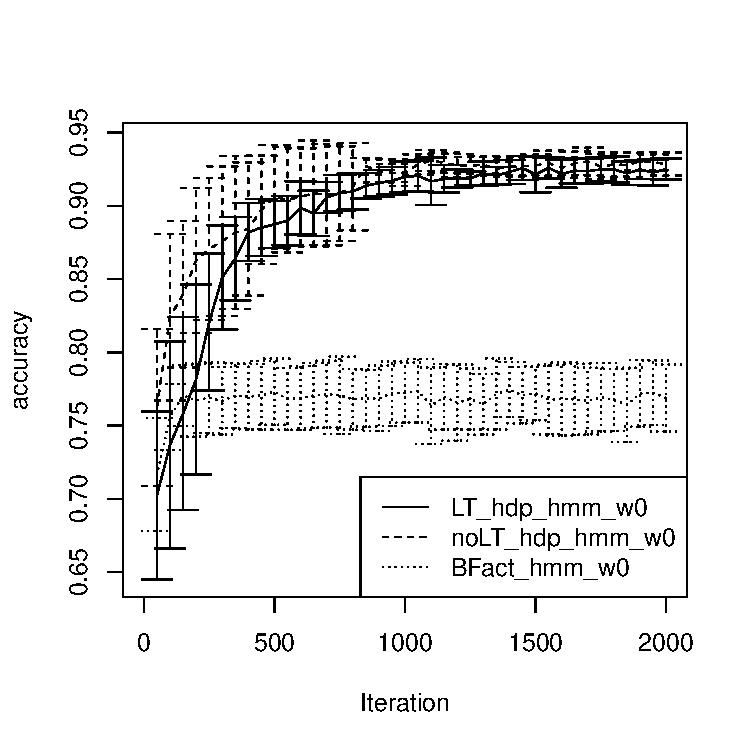
\includegraphics[width =
  \textwidth]{fig/synth16/w0/noLT_s0/accuracy.pdf}
\end{minipage}
\hspace{0.1in}
  \begin{minipage}{0.40\textwidth}
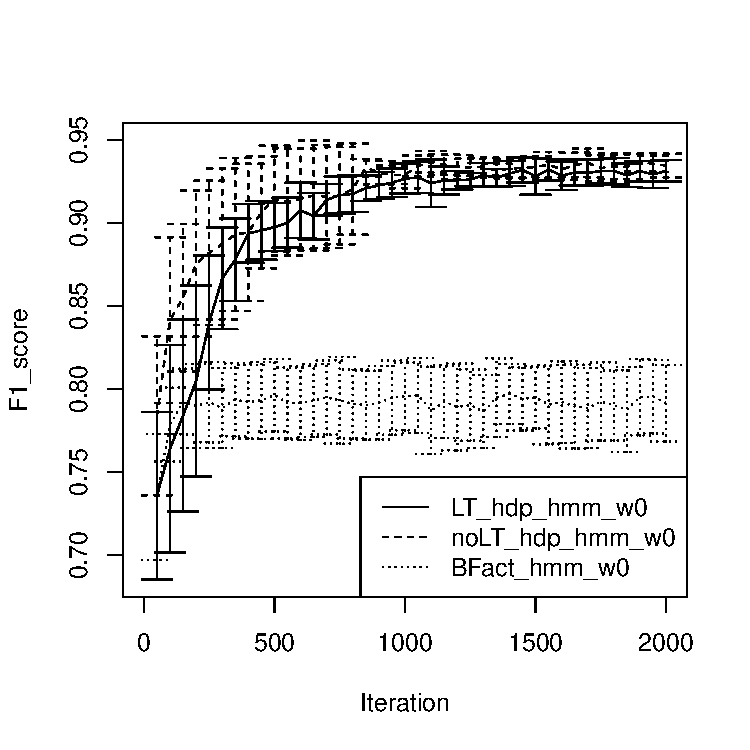
\includegraphics[width = \textwidth]{fig/synth16/w0/noLT_s0/F1_score.pdf}
\end{minipage}

\vspace{-0.3in}

  \begin{minipage}{0.40\textwidth}
  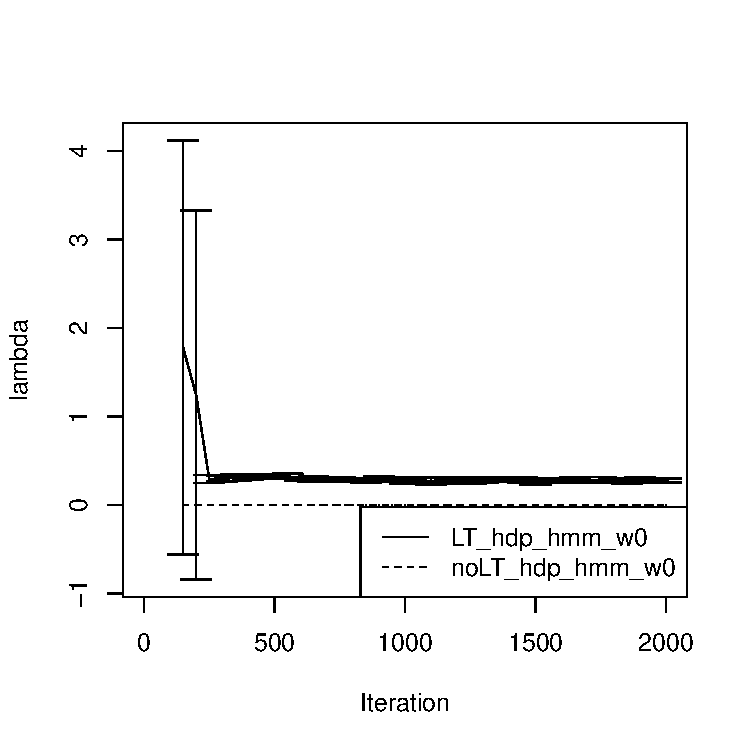
\includegraphics[width = \textwidth]{fig/synth16/w0/noLT_s0/lambda.pdf}
\end{minipage}
  \begin{minipage}{0.40\textwidth}
  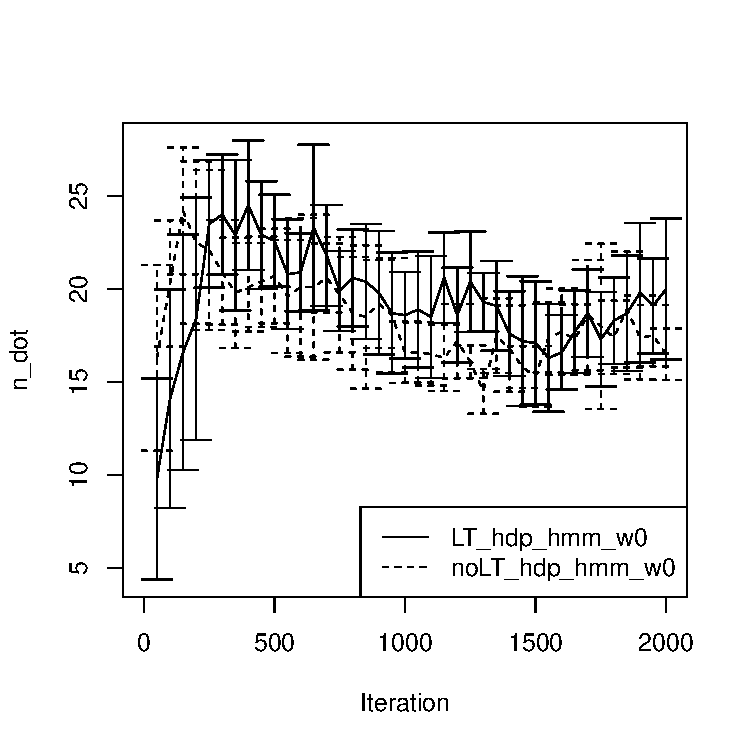
\includegraphics[width = \textwidth]{fig/synth16/w0/noLT_s0/n_dot.pdf}
\end{minipage}
  \caption{(a-b) Accuracy and F1 for the three models on data generated 
    from an HDP-HMM without local transitions, (c) Learned similarity
    parameter, $\lambda$,
  for the LT model, (d) Number of states used by
  the HDP-HMM and HDP-HMM-LT.  The first 100 iterations are omitted.}
  \label{fig:synthetic-results}
\end{figure}
